\documentclass[10pt,a4paper]{article}
\usepackage[margin=2.3cm]{geometry}
\usepackage{fontspec,unicode-math}
\setmainfont{Libertinus Serif}\setsansfont{IBM Plex Sans}\setmonofont[Scale=0.85]{IBM Plex Mono}\setmathfont{Libertinus Math}
\usepackage{amsmath,amsthm,booktabs,tabularx,array,xcolor,enumitem,tikz,hyperref,microtype}
\usetikzlibrary{arrows.meta,positioning,fit}
\renewcommand{\tabularxcolumn}[1]{>{\raggedright\arraybackslash}p{#1}}
\setlength{\emergencystretch}{3em}
\theoremstyle{plain}\newtheorem{theorem}{Theorem}\newtheorem{lemma}{Lemma}\newtheorem{corollary}{Corollary}
\theoremstyle{definition}\newtheorem{definition}{Definition}\newtheorem{assumption}{Assumption}
\theoremstyle{remark}\newtheorem*{remark}{Remark}
\newcommand{\M}{\mathcal{M}}\newcommand{\Pl}{\mathcal{P}}\newcommand{\Lp}{\mathcal{L}}\newcommand{\C}{\mathcal{C}}
\title{\sffamily\bfseries The robot motions implement the experiment\\[4pt]\large Refinement theorems and their proofs for the challenge--rescue experiment on Cell~01}
\author{Generated from the proof checkers' outputs (rsa/refinement\_proof.py, validate\_plan\_z3.py)}
\date{2026-10-18}
\begin{document}\maketitle
\begin{abstract}
The experiment is stated at the culture level: which cultures receive which treatment when, which are observed, and
what must never happen to them. The robots execute motions. This document states, as theorems, that every execution of
the motion-level plan either realizes the culture-level design, in order and under every stated constraint, or is
stopped by a monitor and ends in a failure handler whose guarantee holds. The proof composes seven obligations across
four levels of abstraction; each obligation is discharged by a machine check (z3, the LDL checker, an exhaustive check
over the motions), and each check is shown to be discriminating by negative controls. The result is relative to six
explicit assumptions about controllers, sensors and devices. All quantities are the twin's and ILLUSTRATIVE (D016).
\end{abstract}

\section{Four levels and their abstraction maps}
\begin{center}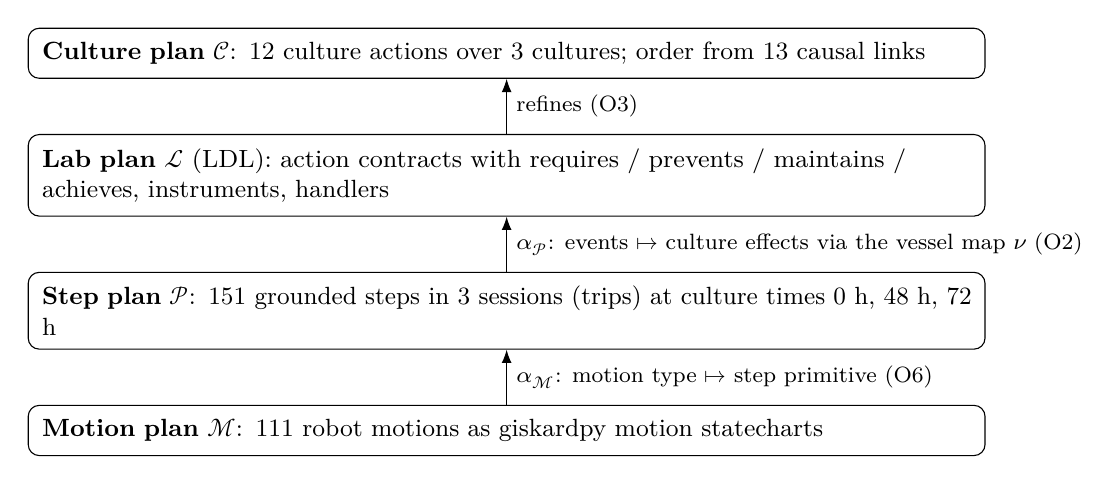
\begin{tikzpicture}[node distance=7mm and 6mm, box/.style={draw, rounded corners, align=left, inner sep=5pt, text width=118mm, font=\small}]
\node[box] (C) {\textbf{Culture plan} $\C$: 12 culture actions over 3 cultures; order from 13 causal links};
\node[box, below=of C] (L) {\textbf{Lab plan} $\Lp$ (LDL): action contracts with requires / prevents / maintains / achieves, instruments, handlers};
\node[box, below=of L] (P) {\textbf{Step plan} $\Pl$: 151 grounded steps in 3 sessions (trips) at culture times 0 h, 48 h, 72 h};
\node[box, below=of P] (M) {\textbf{Motion plan} $\M$: 111 robot motions as giskardpy motion statecharts};
\draw[-{Latex}] (L) -- node[right, font=\footnotesize] {refines (O3)} (C);
\draw[-{Latex}] (P) -- node[right, font=\footnotesize] {$\alpha_{\Pl}$: events $\mapsto$ culture effects via the vessel map $\nu$ (O2)} (L);
\draw[-{Latex}] (M) -- node[right, font=\footnotesize] {$\alpha_{\M}$: motion type $\mapsto$ step primitive (O6)} (P);
\end{tikzpicture}\end{center}


\begin{definition}[Culture plan]\label{def:culture}
$\C = (A_{\C}, \prec_{\C}, \mathit{Eff}_{\C}, \mathit{Prev}_{\C})$: the culture actions $A_{\C}$ with their culture times, the
partial order $\prec_{\C}$ derived from causal links (physical and knowledge effects), the effects $\mathit{Eff}_{\C}$
(a culture exposed to a substance at a dose and time, an observation, an estimate) and the prevented conditions
$\mathit{Prev}_{\C}$ (the control culture is never exposed). The actions are: \texttt{?c1} challenging, \texttt{?c2} challenging, \texttt{?g1} growing, \texttt{?c3} rescuing, \texttt{?g2} growing, \texttt{?o1} observing, \texttt{?o2} observing, \texttt{?o3} observing, \texttt{?i1} interpreting, \texttt{?i2} interpreting, \texttt{?i3} interpreting, \texttt{?a1} analysing.
\end{definition}

\begin{definition}[Vessel map]
$\nu$ maps each culture of $\C$ to the well that holds it:
\begin{center}\small\begin{tabular}{lll}\toprule culture & role & well \\\midrule \texttt{?cr} & rescued & A01 on P17 \\ \texttt{?cc} & comparator & A02 on P17 \\ \texttt{?ck} & control & A05 on P17 \\\bottomrule\end{tabular}\end{center}
\end{definition}

\begin{definition}[Events and the abstraction $\alpha_{\Pl}$]
An execution of $\Pl$ produces events $\mathit{dose}(w, r, q, t)$ (reagent $r$ of $q$ abstract units into well $w$
in the session at culture time $t$) and $\mathit{image}(w, t)$. A culture effect ``$c$ exposed to $r$ at $q$ at $t$''
holds iff $\mathit{dose}(\nu(c), r, q, t)$ occurs; ``$c$ observed at $t$'' holds iff $\mathit{image}(\nu(c), t)$ occurs.
\end{definition}

\begin{definition}[Motion executions and $\alpha_{\M}$]
A motion $m \in \M$ is a statechart that ends either by \emph{EndMotion} (its end monitor true) or by
\emph{CancelMotion} (a cancel condition true). $\alpha_{\M}(m)$ is the step primitive $m$ refines (approach, insert,
grasp, lift, transit, place, release, retract, tool coupling), whose postcondition is that of the step model of
$\Pl$ (Table~\ref{tab:post}).
\end{definition}

\section{Assumptions}

\begin{assumption}[A1] giskardpy semantics: a motion statechart ends only through EndMotion (its end monitor true) or CancelMotion.\end{assumption}
\begin{assumption}[A2] monitor soundness: PoseReached, LocalMinimumReached with the grasp check, VectorsAligned, the collision distance monitors, the simulation clock, the barcode read, the seat sensors and the device monitors observe correctly.\end{assumption}
\begin{assumption}[A3] abstraction: a TCP within 0.4 mm / 0.2 deg of a seat's grasp or release pose has the plate in that seat (the nest guides capture it); within 5 mm of an approach pose it is at that approach pose (free-space waypoint).\end{assumption}
\begin{assumption}[A4] the grasp holds the plate from grasp to release (monitored: grasp\_confirmed, lifted, seating).\end{assumption}
\begin{assumption}[A5] device contracts: dose\_well delivers within its tolerance when its monitors pass; image\_well yields an image when calibration and focus monitors pass; L10 holds the environment profile while the plate is stored.\end{assumption}
\begin{assumption}[A6] the goal frames are the ones the scene defines (rsa/motion\_frames.py), and each is reachable (checked). \end{assumption}
Each assumption is either checked kinematically (A6: 25/25 goal frames reachable),
monitored at run time (A2, A4), part of a device's contract (A5), or the documented semantics of the motion framework (A1).
A3 is a geometric premise: the motion controllers converge to within 0.4 mm, inside the 2 mm capture of the nest guides.


\section{The refinement theorem}
\begin{theorem}[The motions implement the culture-level design]\label{thm:main}
Under A1--A6, every execution $\rho$ of the motion plan $\M$ satisfies exactly one of:
\begin{enumerate}[label=(\roman*)]
\item $\alpha_{\Pl}(\alpha_{\M}(\rho))$ realizes $\C$: every effect of $\mathit{Eff}_{\C}$ occurs at its culture time; the
order $\prec_{\C}$ is respected; $\mathit{Prev}_{\C}$ holds throughout (the control culture is never exposed); and every
stated constraint holds along $\rho$: interlocks, the L12 airspace, identity before use, environment before storing,
calibration before imaging, the 600~s excursion window, contamination freedom, tool hygiene, plate level, collision
distance;
\item a monitor stops $\rho$ (CancelMotion or a device monitor), and $\rho$ ends in a failure handler $h$ whose stated
guarantee $g(h) \in \{\textit{goal}, \textit{goal-or-safe-state}, \textit{safe-state}, \textit{contained}\}$ holds.
\end{enumerate}
\end{theorem}
The proof composes the seven lemmas below (\S\ref{sec:composition}). Status of each, as checked on 2026-10-18:
\begin{center}\small\begin{tabularx}{\linewidth}{@{}lXl@{}}\toprule & obligation & status \\\midrule
O1 & culture plan well formed & \textcolor{green!40!black}{holds} \\
O2 & abstraction: motion-level effects entail the culture plan & \textcolor{green!40!black}{holds} \\
O3 & lab plan: order, threats, instruments, handlers, guarantees & \textcolor{green!40!black}{holds} \\
O4 & step level: executability, safety, time, realization (z3 V1-V5) & \textcolor{green!40!black}{holds} \\
O5 & step level: cleanliness & \textcolor{green!40!black}{holds} \\
O6 & motion refinement: 111 Giskard motions & \textcolor{green!40!black}{holds} \\
O7 & failure branch: every cancellation reaches a guaranteed handler & \textcolor{green!40!black}{holds} \\\bottomrule\end{tabularx}\end{center}


\section{Lemmas and their proofs}
\begin{lemma}[O1: the culture plan is well formed]
Every precondition of every culture action is supported by a causal link from an earlier action's effect or by the
initial state, or is to be established by the executive; the link graph is acyclic.
\end{lemma}
\begin{proof}
\texttt{rsa/culture\_plan.derive} computes, for each requirement, its supporting effects. It finds 13 links, no unsupported requirement and no cycle; the requirements left to establish are 3 known image scales (calibration), which the step level discharges (V2, S3).
$\prec_{\C}$ is the transitive closure of the links, hence a strict partial order.
\end{proof}

\begin{lemma}[O2: the step events entail the culture plan]\label{lem:abs}
Let $E$ be the set of events the step plan provably produces (Theorem~V4 below). Then for each culture obligation
$\varphi$ (each effect of $\mathit{Eff}_{\C}$ at its time, the prevented condition, and the order),
$E \cup \{\text{definition of }\alpha_{\Pl},\ \nu\} \models \varphi$.
\end{lemma}
\begin{proof}
Encode each event as a Boolean fact asserted true and each obligation $\varphi$ as the disjunction of the events that
support it under $\nu$. For each $\varphi$, z3 shows $E \wedge \neg\varphi$ unsatisfiable. The obligations and verdicts:
\begin{center}\small\begin{tabularx}{\linewidth}{@{}Xl@{}}\toprule obligation & $E \wedge \neg\varphi$ \\\midrule
?c1 challenging ?cr: exposed to challenge 0.85 au at 0 h & UNSAT \\
?c2 challenging ?cc: exposed to challenge 0.85 au at 0 h & UNSAT \\
?g1 growing 0 $\to$ 48 h: cultures in their environment between the trips & UNSAT \\
?c3 rescuing ?cr: exposed to rescue 0.70 au at 48 h & UNSAT \\
?g2 growing 48 $\to$ 72 h: cultures in their environment between the trips & UNSAT \\
?o1 observing ?cr: image at 72 h & UNSAT \\
?o2 observing ?cc: image at 72 h & UNSAT \\
?o3 observing ?ck: image at 72 h & UNSAT \\
?i1 interpreting ?cr: image and known scale & UNSAT \\
?i2 interpreting ?cc: image and known scale & UNSAT \\
?i3 interpreting ?ck: image and known scale & UNSAT \\
?a1 analysing: estimates of the rescued, comparator and control cultures & UNSAT \\
prevents: the control culture is never exposed & UNSAT \\
order: challenges at 0 h $<$ rescue at 48 h $<$ observations at 72 h & UNSAT
\\\bottomrule\end{tabularx}\end{center}
The events used are the doses {'s0': [['a01', 'challenge', 85], ['a02', 'challenge', 85]], 's1': [['a01', 'rescue', 70]], 's2': []} (session $\mapsto$ [well, reagent, dose $\times 100$]) and
images of ['a01', 'a02', 'a05'] at {'s0': 0, 's1': 48, 's2': 72}.
\end{proof}

\begin{lemma}[O3: the lab plan refines the culture plan]
The LDL lab plan preserves $\prec_{\C}$; every threat to a causal link is resolved; every instrument role is filled by a
device that offers the slot and the process; every signalled failure has a handler whose guarantee holds.
\end{lemma}
\begin{proof}
By the LDL checker (\texttt{rsa/ldl.py}, \texttt{rsa/ldl\_trust.py}): order preserved from culture to lab level: True; threats resolved 9/9; repair guarantees 13/13; its negative controls caught 12/12. A guarantee \textit{goal} is admitted only if the fault is detected before the process's irreversible phase and is transient or removed by what the handler re-establishes; \textit{safe-state} only if the handler escalates or abstains, the plate is restorable, nothing is committed and evidence is kept.
\end{proof}


\begin{theorem}[O4: the step plan is executable, safe, timely and realizes the design]\label{thm:steps}
Each trip of the step plan is unrolled into z3 state variables (plate location, each robot's position and gripper,
R02's tool, the L10 shuttle and L17 stage, L12's tip and reagent, environment, QC and identity flags), one transition
per step. Then:
\begin{description}[leftmargin=2em, style=nextline]
\item[V1 executability and preservation] every step's precondition holds and each trip ends with the plate at home,
grippers empty and no robot in a seat, for every initial tool and stage state;
\item[V2 safety] S1 no L12 operation while a robot is in the deck seat; S2 environment checked before storing; S3 image
only with valid calibration or after QC; S6 interlocks closed; S7 identity verified first;
\item[V3 time] every trip fits the 600~s window for all step durations within $\pm 20\,\%$ of the estimates;
\item[V4 realization] the doses and images are exactly those the selected design requires, in sessions at
$t_0$, $t_0 + 48$~h, $t_0 + 72$~h; arms disjoint with a control (V4b);
\item[V5 gain and cost] the design's expected information gain meets the requirement, and no cheaper design does.
\end{description}
\end{theorem}
\begin{proof}
For each claim $\psi$, z3 shows $\mathit{Trans} \wedge \neg\psi$ unsatisfiable, where $\mathit{Trans}$ is the
conjunction of the transitions (\texttt{validate\_plan\_z3.py}, an encoding separate from the answer-set program that
derived the plan). Results:
\begin{center}\small\begin{tabularx}{\linewidth}{@{}Xll@{}}\toprule claim & result & checked \\\midrule
V1 executability / preservation & \textcolor{green!40!black}{holds} & 278 \\
V2 safety S1 S2 S3 S6 S7 & \textcolor{green!40!black}{holds} & 115 \\
V3 time window (S5), durations +-20 \% & \textcolor{green!40!black}{holds} & 3 \\
V4 realisation (doses, images, session times) & \textcolor{green!40!black}{holds} &  \\
V4b arms E2M3 + control S9 & \textcolor{green!40!black}{holds} &  \\
V5 gain met (EIG $>$= g) & \textcolor{green!40!black}{holds} & 0.5439 \\
V5b least cost, then max EIG, over all candidates meeting g & \textcolor{green!40!black}{holds} & 13
\\\bottomrule\end{tabularx}\end{center}
Ten mutated plans, each breaking one claim, are each caught (satisfiable negation) by the expected theorem: N1 retract after the first L12 tip pick, N2 environment wait removed, N3 L17 calibration expired, no QC step, N4 identity check removed, N5 R02 transit to L12 removed, N6 tool change removed (initial tool unknown), N7 challenge dose changed (0.85 $\to$ 0.65 au), N8 selected candidate below the requirement, N9 window shortened to 250 s, N10 control well not imaged.
\end{proof}

\begin{lemma}[O5: cleanliness]
No tool that touches a culture is ever used to handle the plate, and contamination freedom is a requirement of every
dosing and imaging step.
\end{lemma}
\begin{proof}
The plate-handling tools used are t01; the tools that touch cultures are t03, t04. z3 shows that asserting any used tool to touch a culture contradicts the facts. contamination\_free is in the constraint registry: True.
\end{proof}


\begin{lemma}[O6: every motion refines its step]\label{lem:motion}
For each of the 111 motions $m$: (a) $m$'s type refines the step primitive $\alpha_{\M}(m)$;
(b) if $m$ ends by EndMotion, the postcondition of $\alpha_{\M}(m)$ holds (under A3, A4); (c) while the plate is held,
tilt beyond the level tolerance cancels $m$; (d) a violated collision distance cancels $m$; (e) $m$ is cancelled if it
runs longer than $1.2\times$ its estimated duration, which is the duration bound V3 assumes.
\end{lemma}
\begin{proof}
Exhaustive check over the motions (\texttt{refinement\_proof.motion\_proof}) against the end monitors and their
tolerances (Table~\ref{tab:post}); each end tolerance is at most the capture of the seat it acts on (0.4~mm $\le$ 2~mm
for seats, 5~mm for free-space approach poses, 4~mm lock gap for the coupler), so by A3 EndMotion implies the
postcondition. The generated controller code contains the cancel conditions (timeout: True, tilt: True, collision: True). Result: 111/111 motions
satisfy (a)--(e); goal frames reachable 25/25.
\begin{table}[h]\centering\footnotesize\caption{Motion types, the steps they refine, and why their end monitor implies
the step's postcondition.}\label{tab:post}
\begin{tabularx}{\linewidth}{@{}lrllXX@{}}\toprule motion & n & step & postcondition & end monitor & why \\\midrule
aligning & 12 & approach & pos = appr(seat) & PoseReached & A3: within 0.4 mm / 0.2 deg of the approach pose \\
approaching & 12 & approach & pos = appr(seat) & CartesianPose observation & A3: within 5 mm of the approach pose \\
coupling & 3 & tool\_couple & tool = T01 & PoseReached within the lock gap & A2: the coupler locks within 4 mm \\
grasping & 12 & grasp & grip and plate = robot & LocalMinimumReached + grasp\_confirmed & A4: the jaws stalled on the plate, contact and lift confirmed \\
inserting & 12 & insert & pos = seat & PoseReached & A3: within 0.4 mm / 0.2 deg of the grasp pose, the plate between the jaws \\
lifting & 12 & lift & pos = appr(seat), plate held & CartesianPositionStraight observation & A3 + A4: at the approach height, plate held \\
placing & 12 & place & pos = seat, plate = seat & CartesianPositionStraight observation & A3: at the release height over the seat; the guides capture the plate \\
releasing & 12 & release & not grip & LocalMinimumReached & A2: the jaws open \\
retracting & 12 & retract & pos = appr(seat) & CartesianPositionStraight observation & A3: back at the approach height \\
transiting & 12 & transit & pos = appr(target) & CartesianPose observation & A3: within 5 mm of the target approach pose
\\\bottomrule\end{tabularx}\end{table}
\end{proof}

\begin{lemma}[O7: every stop ends in a guaranteed handler]
Every CancelMotion (timeout, tilt, collision) and every device monitor's failure reaches a handler of the experiment
whose stated guarantee holds.
\end{lemma}
\begin{proof}
A cancelled motion raises MotionContractViolated (or CollisionViolatedError); it propagates to the session, whose
unwind-protect returns the plate to its home; the handler for a violated \textit{prevents} item guarantees a safe state.
Device monitors signal the failure types of the process models, each with its own handler. The guarantees checked
(O3) are: identity-mismatch: ok, measurement-invalid/calibration\_expired: ok, measurement-invalid/out\_of\_focus: ok, measurement-invalid/plate\_misseated: ok, validity-effect-unachievable: ok, dose-not-delivered/wrong\_reagent: ok, dose-not-delivered/tip\_missing\_or\_dropped: ok, dose-not-delivered/clog\_or\_air\_aspiration: ok, dose-not-delivered/well\_misregistration: ok, contamination-suspected: ok, environment-excursion: ok, containment-breach: ok, prevents-violated: ok.
\end{proof}


\section{Proof of Theorem~\ref{thm:main}}\label{sec:composition}
\begin{proof}
Let $\rho$ be an execution of $\M$. By A1 each motion of $\rho$ ends by EndMotion or by CancelMotion; device steps end
with their monitors passing or a failure signalled (A5).

\emph{Case 1: no motion is cancelled and no device monitor fails.} By Lemma~\ref{lem:motion}(b), after each motion the
postcondition of its step holds; device steps achieve their contract effects (A5). Hence $\alpha_{\M}(\rho)$ is an
execution of the step plan in which each step's effect holds when it ends. By Theorem~\ref{thm:steps} (V1) the
precondition of every next step then holds, so $\alpha_{\M}(\rho)$ is a complete execution of $\Pl$; by V2 the safety
constraints S1, S2, S3, S6, S7 hold along it; by Lemma~\ref{lem:motion}(e) every duration is within $1.2\times$ its
estimate, so V3 applies and each trip keeps the 600~s window; by Lemma~\ref{lem:motion}(c, d) the plate stays level and
no collision distance is violated; by O5 no culture-touching tool handles the plate. By V4 the events of the execution
are exactly $E$. By Lemma~\ref{lem:abs}, $E$ entails every culture effect at its time, the order, and that the control
culture is never exposed. By O1 and O3 these effects, in this order, are the culture plan and its lab-level refinement.
So (i) holds.

\emph{Case 2: some motion is cancelled or a device monitor fails.} The first such event stops the trip; by O7 it reaches
a handler whose guarantee holds. So (ii) holds.

The cases are exhaustive by A1 and A5, and exclusive because (i) requires a complete execution. \qedhere
\end{proof}

\begin{corollary}
The design's purpose is preserved: the comparisons the experiment makes (rescued vs comparator, comparator vs control)
are between cultures that received exactly the designed treatments, so any conclusion drawn from an execution in case
(i) is about the designed contrast; in case (ii) no conclusion is drawn (the handler commits nothing).
\end{corollary}

\section{The checks discriminate: negative controls}
Each mutation must make an obligation fail; a check that passes a mutant would prove nothing.
\begin{center}\small\begin{tabularx}{\linewidth}{@{}Xl@{}}\toprule mutation & caught \\\midrule
vessel map swaps rescued and comparator & yes \\
the control well A05 is also dosed & yes \\
the control well is not imaged & yes \\
the plate tool T01 touches the culture & yes \\
one held motion without the tilt cancel & yes \\
one motion's timeout beyond V3's bound (1.5 x) & yes \\
a motion that does not refine its step & yes \\
step level: the validator's own 10 mutated plans & yes
\\\bottomrule\end{tabularx}\end{center}

\section{Scope and what is not proved}
\begin{itemize}
\item \textbf{The current design only.} The theorem is about the selected plan (three cultures, one well each). The
improved five-arm design has no derived step and motion plan yet; its proof needs the same chain (derive the plan,
V1--V5, O2 with its 15 units and the vehicle doses, O6).
\item \textbf{Progress.} The plan may stop (case ii) rather than finish; no probability of finishing is claimed.
\item \textbf{Partially detected faults.} L12 well misregistration and L17 plate misseating are detected only partly
(6 of 27 fault instances); for these, case (ii) is not guaranteed.
\item \textbf{The imaging postcondition (new, 2026-10-18).} A5 reads ``image\_well yields an image of the well when
calibration and focus monitors pass''. The L17 twin without plate registration places its 4$\times$ field 0.2--0.65~mm
from the well centre and misses the organoid in 3 of 5 wells. When the field contains no structure, focus fails and case
(ii) applies; a field that shows debris but not the organoid could pass and violate A5 silently. Edge-finding plate
registration (\texttt{L17Controller.register\_plate}, in progress) is meant to discharge this premise; until it is
verified, A5 for imaging is a premise, not a fact of the twin.
\item \textbf{Physics and execution.} Compliant insertion is not modelled; the Giskard module is generated and checked
but not run (no SDT world for it); R02 is not collision-checked offline.
\item \textbf{Biology.} The goal is an expected information gain under the surrogate model, not a biological finding.
\end{itemize}
\end{document}
